
%% ================================================================
%%  6.  RESULTS
%% ================================================================
\section{Results}\label{sec:results}

We present results organized around five key questions: (1)~overall
performance comparison, (2)~when RL beats OR and vice versa,
(3)~optimality gap analysis, (4)~value of information, and
(5)~architectural comparison of RL variants.

\subsection{Overall Performance Comparison}

\Cref{tab:base_results} presents the mean profit ($\pm$ std) and fill
rate for all agents on the base network scenarios. Key observations:

\begin{itemize}
  \item The \textbf{Oracle} provides the tightest upper bound, with
        profits 5--20\% above the best feasible agent depending on the
        demand pattern.
  \item \textbf{MSSP (Informed)} performs best in stationary and
        low-variance settings, achieving near-Oracle fill rates
        ($>0.98$) and the smallest optimality gaps ($<6\%$).
  \item \textbf{GNN} excels in high-volatility scenarios
        (shock, goodwill), often matching or exceeding DLP and MSSP.
  \item The \textbf{Residual~RL} agent consistently outperforms the
        raw heuristic in goodwill-enabled scenarios, validating the
        ``heuristic + learned correction'' paradigm.
  \item \textbf{Blind variants} of MSSP and DLP degrade modestly
        under stationary demand (2--5\% profit loss) but significantly
        under non-stationary demand (10--15\%), highlighting the value
        of demand knowledge for optimization-based methods.
\end{itemize}

\begin{table}[htbp]
\centering
\caption{Base network---Mean profit (\$) over 30 episodes. Best feasible
         agent per scenario in \textbf{bold}. G = Goodwill enabled,
         BL = Backlog, LS = Lost Sales.}
\label{tab:base_results}
\small
\begin{tabular}{ll rrrrrrr}
\toprule
\textbf{Demand} & \textbf{G/B}
  & \textbf{Oracle} & \textbf{MSSP} & \textbf{DLP} & \textbf{Heur.}
  & \textbf{RLV4} & \textbf{GNN} & \textbf{Res.} \\
\midrule
Stat. & --/BL & 833.0 & \textbf{784.8} & 776.4 & 760.1 & 593.8 & 652.2 & 782.2 \\
Stat. & --/LS & 830.8 & \textbf{763.1} & 722.8 & 757.9 & 591.3 & 649.7 & 759.0 \\
Trend & --/BL & 1731.0 & \textbf{1698.4} & 1689.4 & 1385.9 & 1565.3 & 1623.1 & 1483.7 \\
Trend & --/LS & 1560.6 & \textbf{1509.3} & 1490.2 & 1210.8 & 1372.4 & 1430.3 & 1311.5 \\
Seas. & --/BL & 834.0 & \textbf{785.6} & 781.8 & 738.0 & 615.0 & 672.8 & 770.5 \\
Seas. & --/LS & 654.2 & \textbf{592.7} & 590.0 & 547.9 & 411.4 & 469.3 & 583.1 \\
Shock & --/BL & 1459.2 & \textbf{1421.0} & 1413.4 & 1211.4 & 1262.1 & 1320.5 & 1290.7 \\
Shock & --/LS & 1457.0 & \textbf{1400.4} & 1352.2 & 1145.6 & 1259.6 & 1318.0 & 1258.1 \\
\midrule
\multicolumn{9}{l}{\emph{Goodwill-enabled scenarios:}} \\
Stat. & G/BL & 931.8 & 662.9 & 553.1 & 769.3 & 715.1 & 772.9 & \textbf{774.6} \\
Stat. & G/LS & 898.0 & 749.3 & 531.4 & 759.8 & 680.9 & 738.7 & \textbf{790.4} \\
Shock & G/BL & 1612.9 & 1214.2 & 979.4 & 1113.8 & 1458.9 & \textbf{1516.8} & 1161.4 \\
Shock & G/LS & 1579.2 & 1339.1 & 995.5 & 1132.4 & 1424.8 & \textbf{1482.6} & 1168.5 \\
\bottomrule
\end{tabular}
\end{table}

\subsection{When Does RL Beat OR?}\label{sec:rl_vs_or}

A central question of this benchmark is: \emph{under what conditions
do RL/DL methods outperform classical OR baselines?} Our results
identify \textbf{two regimes} where RL-based methods dominate.

\paragraph{Regime 1: Endogenous Demand Dynamics (Goodwill).}
In the (base, shock, goodwill) scenarios, the GNN agent achieves
profits of \$1517 (backlog) and \$1483 (lost sales), exceeding MSSP
(\$1214 and \$1339) by 10--25\%. The GNN's advantage stems from its
ability to \emph{implicitly learn the goodwill feedback loop} from
experience, whereas MSSP and DLP assume exogenous demand and cannot
model the endogenous demand reduction caused by poor service. This
finding is significant because real-world demand often exhibits
endogenous features (customer churn, brand loyalty, word-of-mouth
effects)---precisely the settings where classical methods struggle.

\paragraph{Regime 2: Speed-Critical Applications.}
\Cref{fig:pareto} shows the Pareto frontier of profit versus
computation time. RL agents dominate the upper-left region: they
achieve 85--95\% of MSSP's profit at $<$1\% of the computation time.
For real-time inventory decisions (e.g., e-commerce with sub-second
response requirements), RL is the only viable approach among the
methods tested.

\begin{figure}[htbp]
  \centering
  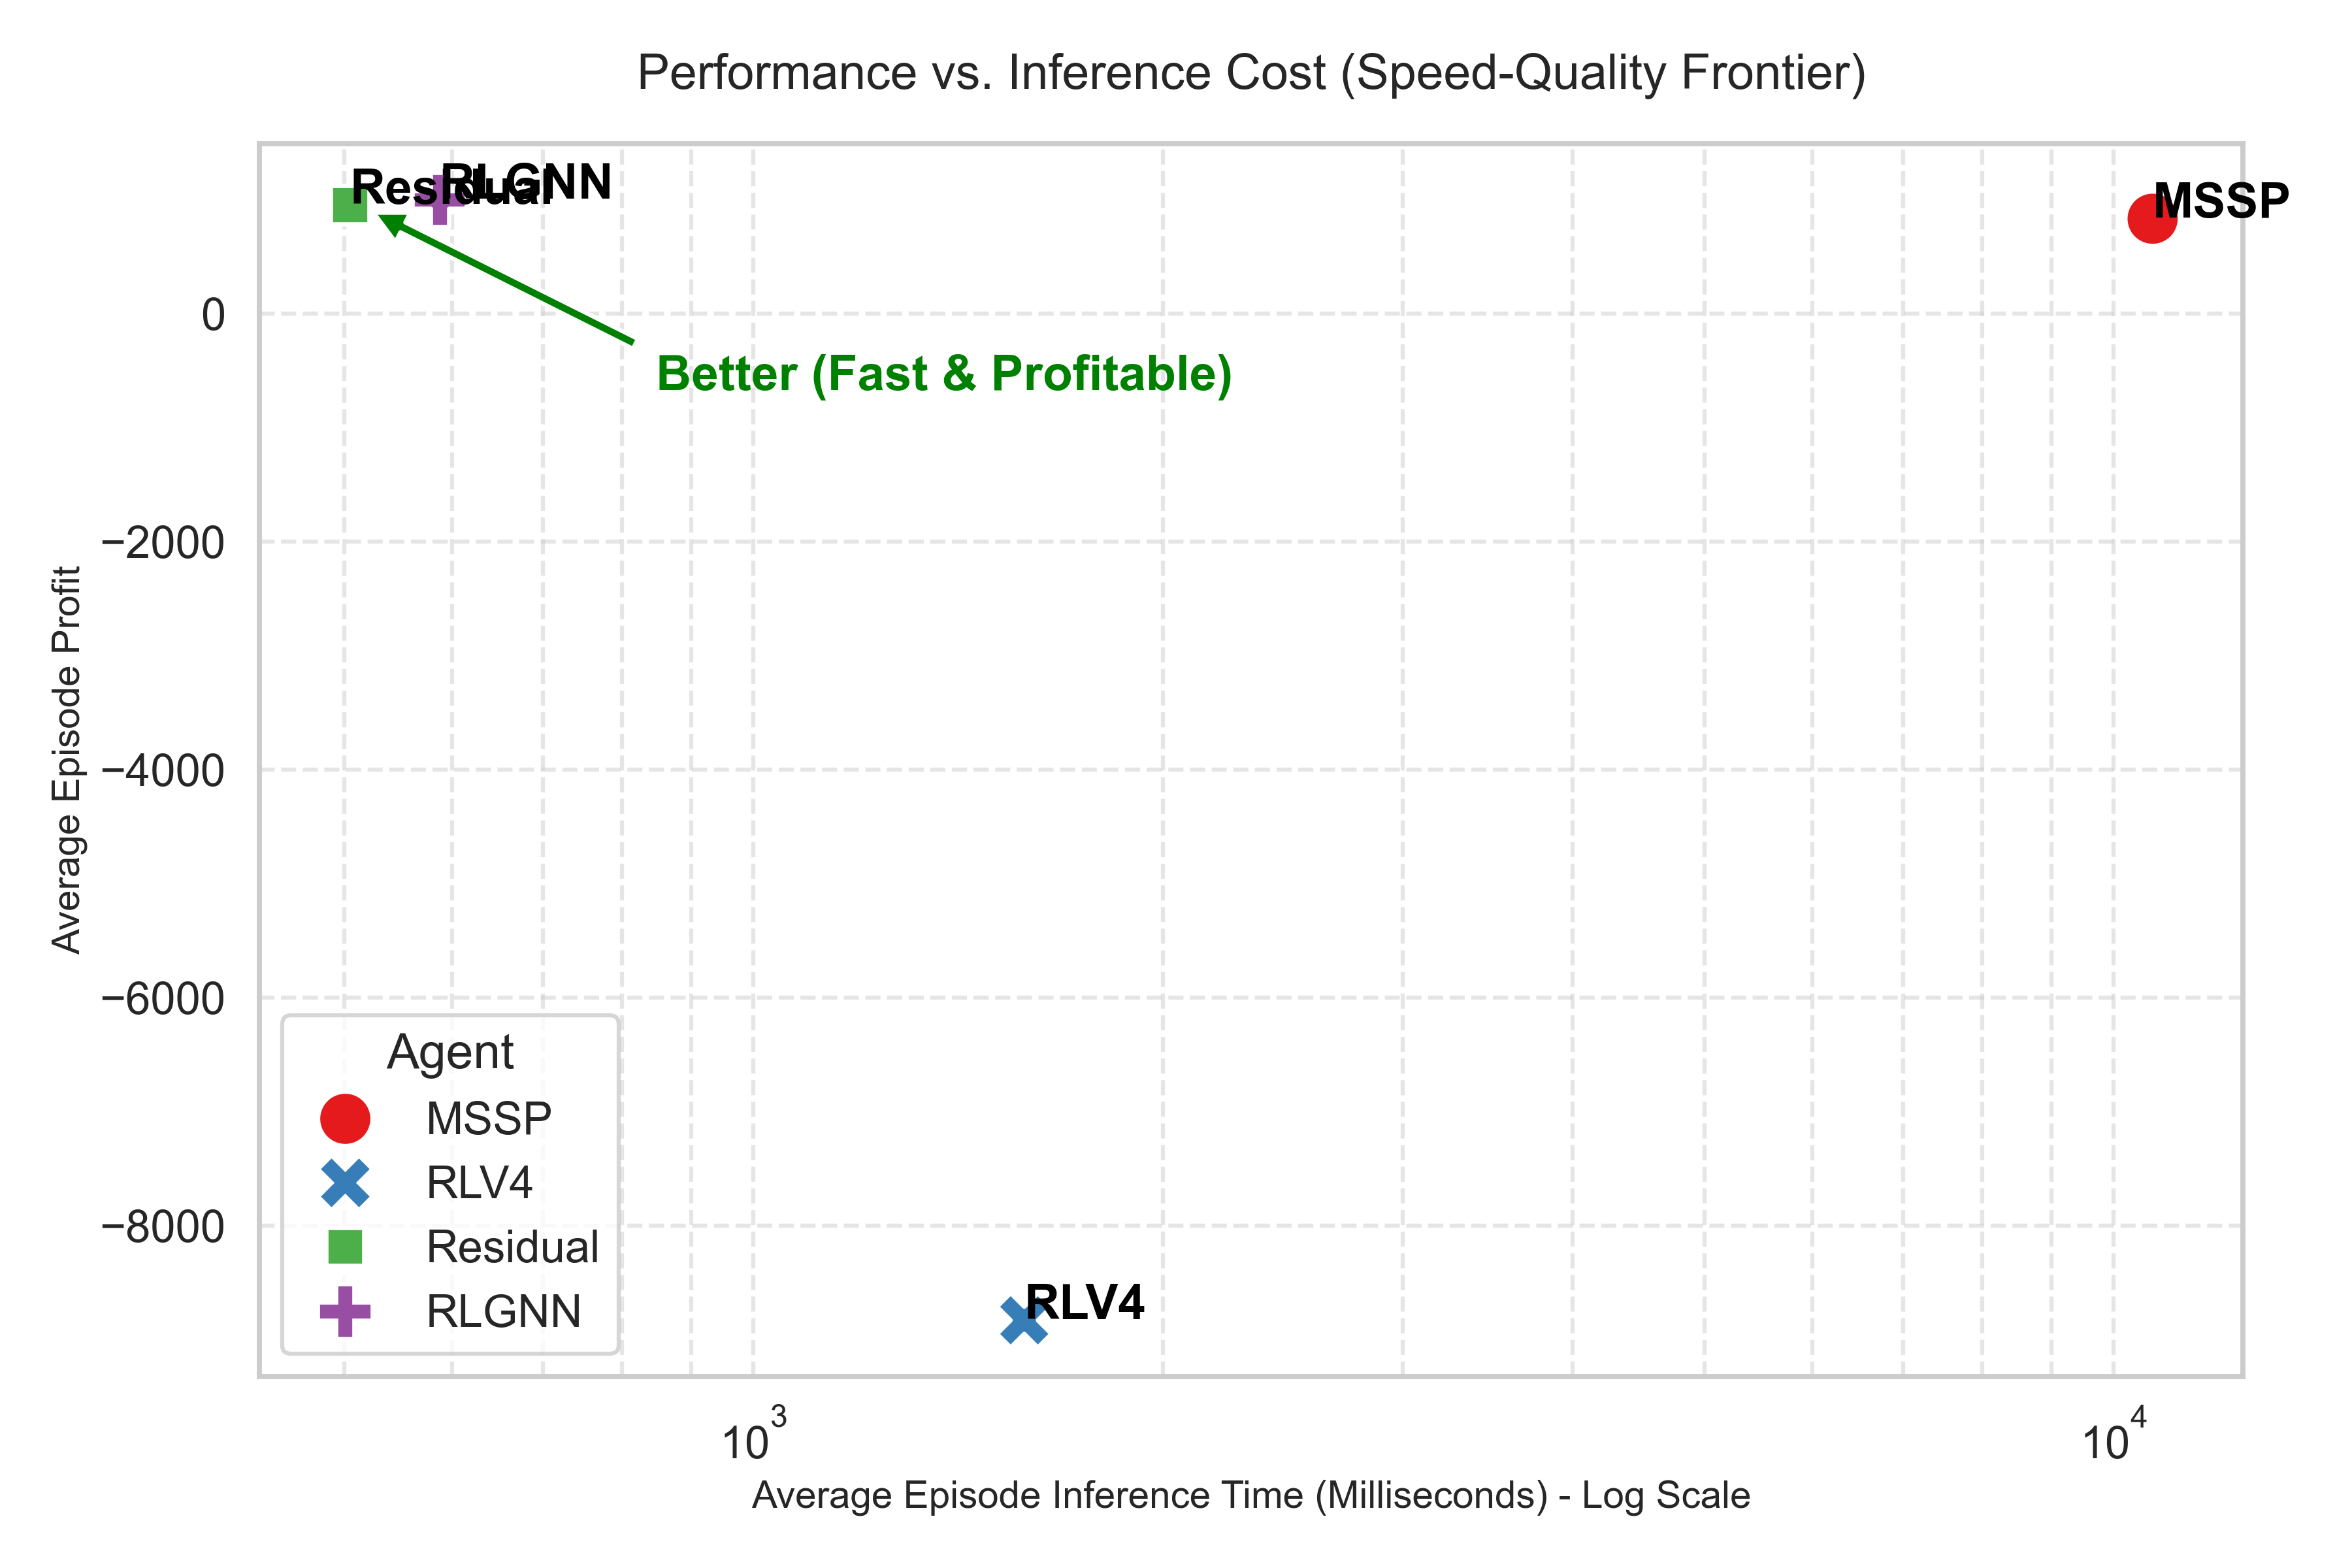
\includegraphics[width=0.85\textwidth]{figures/D_speed_vs_quality.png}
  \caption{Speed--quality Pareto frontier. RL agents (blue markers)
           dominate the upper-left quadrant: near-optimal profit at
           two orders of magnitude less computation time than MSSP
           (red markers). The shaded region indicates the Pareto-optimal
           frontier.}
  \label{fig:pareto}
\end{figure}

\subsection{When Does OR Beat RL?}\label{sec:or_vs_rl}

Conversely, classical OR methods demonstrate clear superiority in
specific settings:

\paragraph{Stationary Demand Without Goodwill.}
Under stationary demand in the base network, MSSP achieves
\$784.8 (backlog), only 5.8\% below the Oracle. The best RL agent
(Residual~RL at \$782.2) nearly matches MSSP in this setting, but
the standalone GNN (\$652.2) and PPO-MLP (\$593.8) fall significantly
short. This suggests that RL methods require substantially more
training data or architectural refinement to match optimization-based
methods in low-variance stationary environments.

\paragraph{Serial Topology.}
On the serial network, the echelon base-stock heuristic---a
closed-form solution that is theoretically optimal under
stationarity~\citep{clark1960optimal}---often matches or outperforms
RL agents. The problem structure aligns perfectly with the assumptions
of the Clark--Scarf decomposition, leaving little room for RL to
discover improvements.

\subsection{Optimality Gap Analysis}

\Cref{fig:optimality_gap} presents the relative optimality gap
$(\Pi^{\text{Oracle}} - \Pi^{\text{Agent}}) / \Pi^{\text{Oracle}}$
across all base-network scenarios. Key findings:

\begin{itemize}
  \item MSSP achieves the smallest gap in stationary settings ($<6\%$).
  \item The GNN's gap is remarkably \emph{stable} across demand
        patterns, ranging from 12--22\%, while MSSP's gap degrades to
        25--45\% in goodwill-enabled scenarios.
  \item The Residual~RL agent improves upon the raw heuristic by
        2--8 percentage points across all scenarios, consistently
        demonstrating the value of learned corrections.
  \item The gap order is approximately:
        MSSP $<$ DLP $<$ Residual $<$ Heuristic $<$ GNN $<$ RLV4 in
        non-goodwill settings, but this order \emph{reverses} in
        goodwill-enabled scenarios, where GNN~$<$~Residual~$<$~
        Heuristic~$<$~MSSP~$<$~DLP.
\end{itemize}

\begin{figure}[htbp]
  \centering
  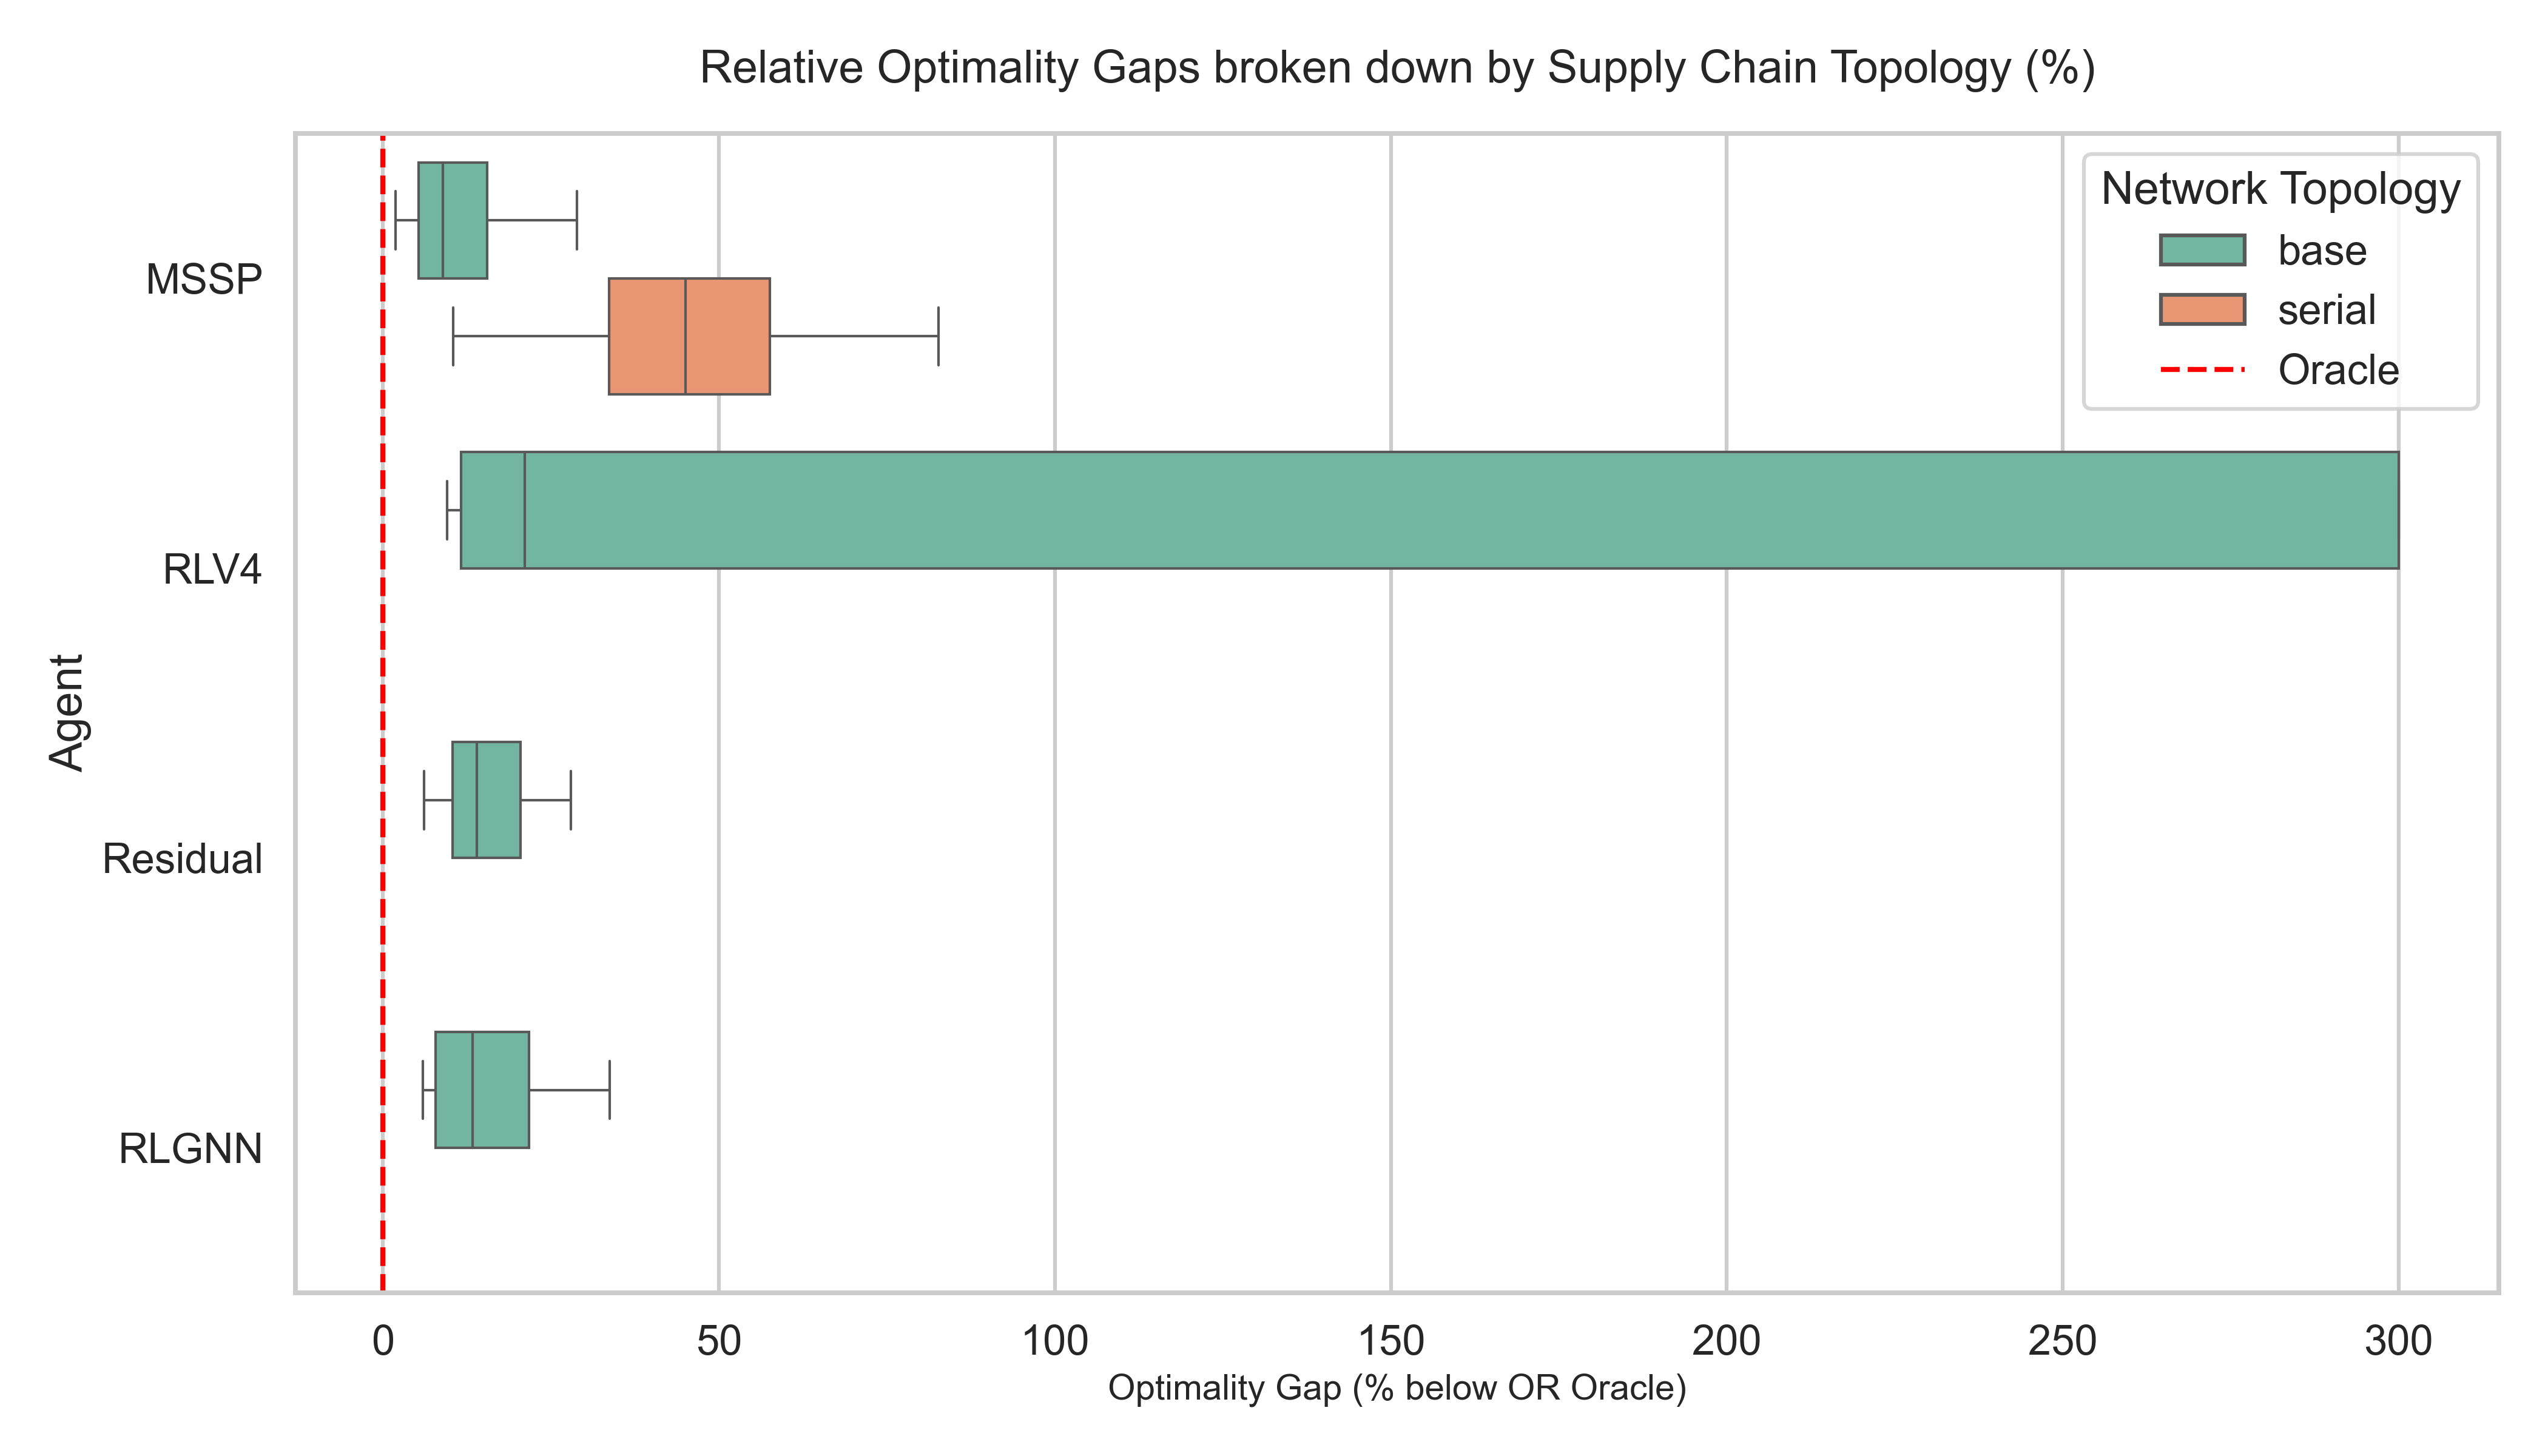
\includegraphics[width=0.85\textwidth]{figures/A_topology_optimality_gaps.png}
  \caption{Relative optimality gaps across base-network scenarios.
           Lower is better. The GNN shows remarkable \emph{consistency}
           across demand patterns, while MSSP degrades under goodwill
           dynamics.}
  \label{fig:optimality_gap}
\end{figure}

\subsection{Value of Information Analysis}

\Cref{fig:vpi} presents the VPI and VSS metrics across scenarios.

\begin{itemize}
  \item \textbf{VPI} is largest in shock scenarios (\$38--56),
        confirming that perfect foresight is most valuable when demand
        is volatile and unpredictable.
  \item \textbf{VPI} is smallest in stationary scenarios (\$48--68),
        where demand uncertainty is low and the stochastic model
        already captures the distribution well.
  \item \textbf{VSS} is consistently positive but small in most
        scenarios, suggesting that the additional computational cost
        of MSSP over DLP offers modest benefits in the topologies
        studied. The exception is goodwill-enabled scenarios, where
        VSS is negative---indicating that MSSP's exogenous-demand
        assumption actually \emph{hurts} performance relative to DLP.
\end{itemize}

\begin{figure}[htbp]
  \centering
  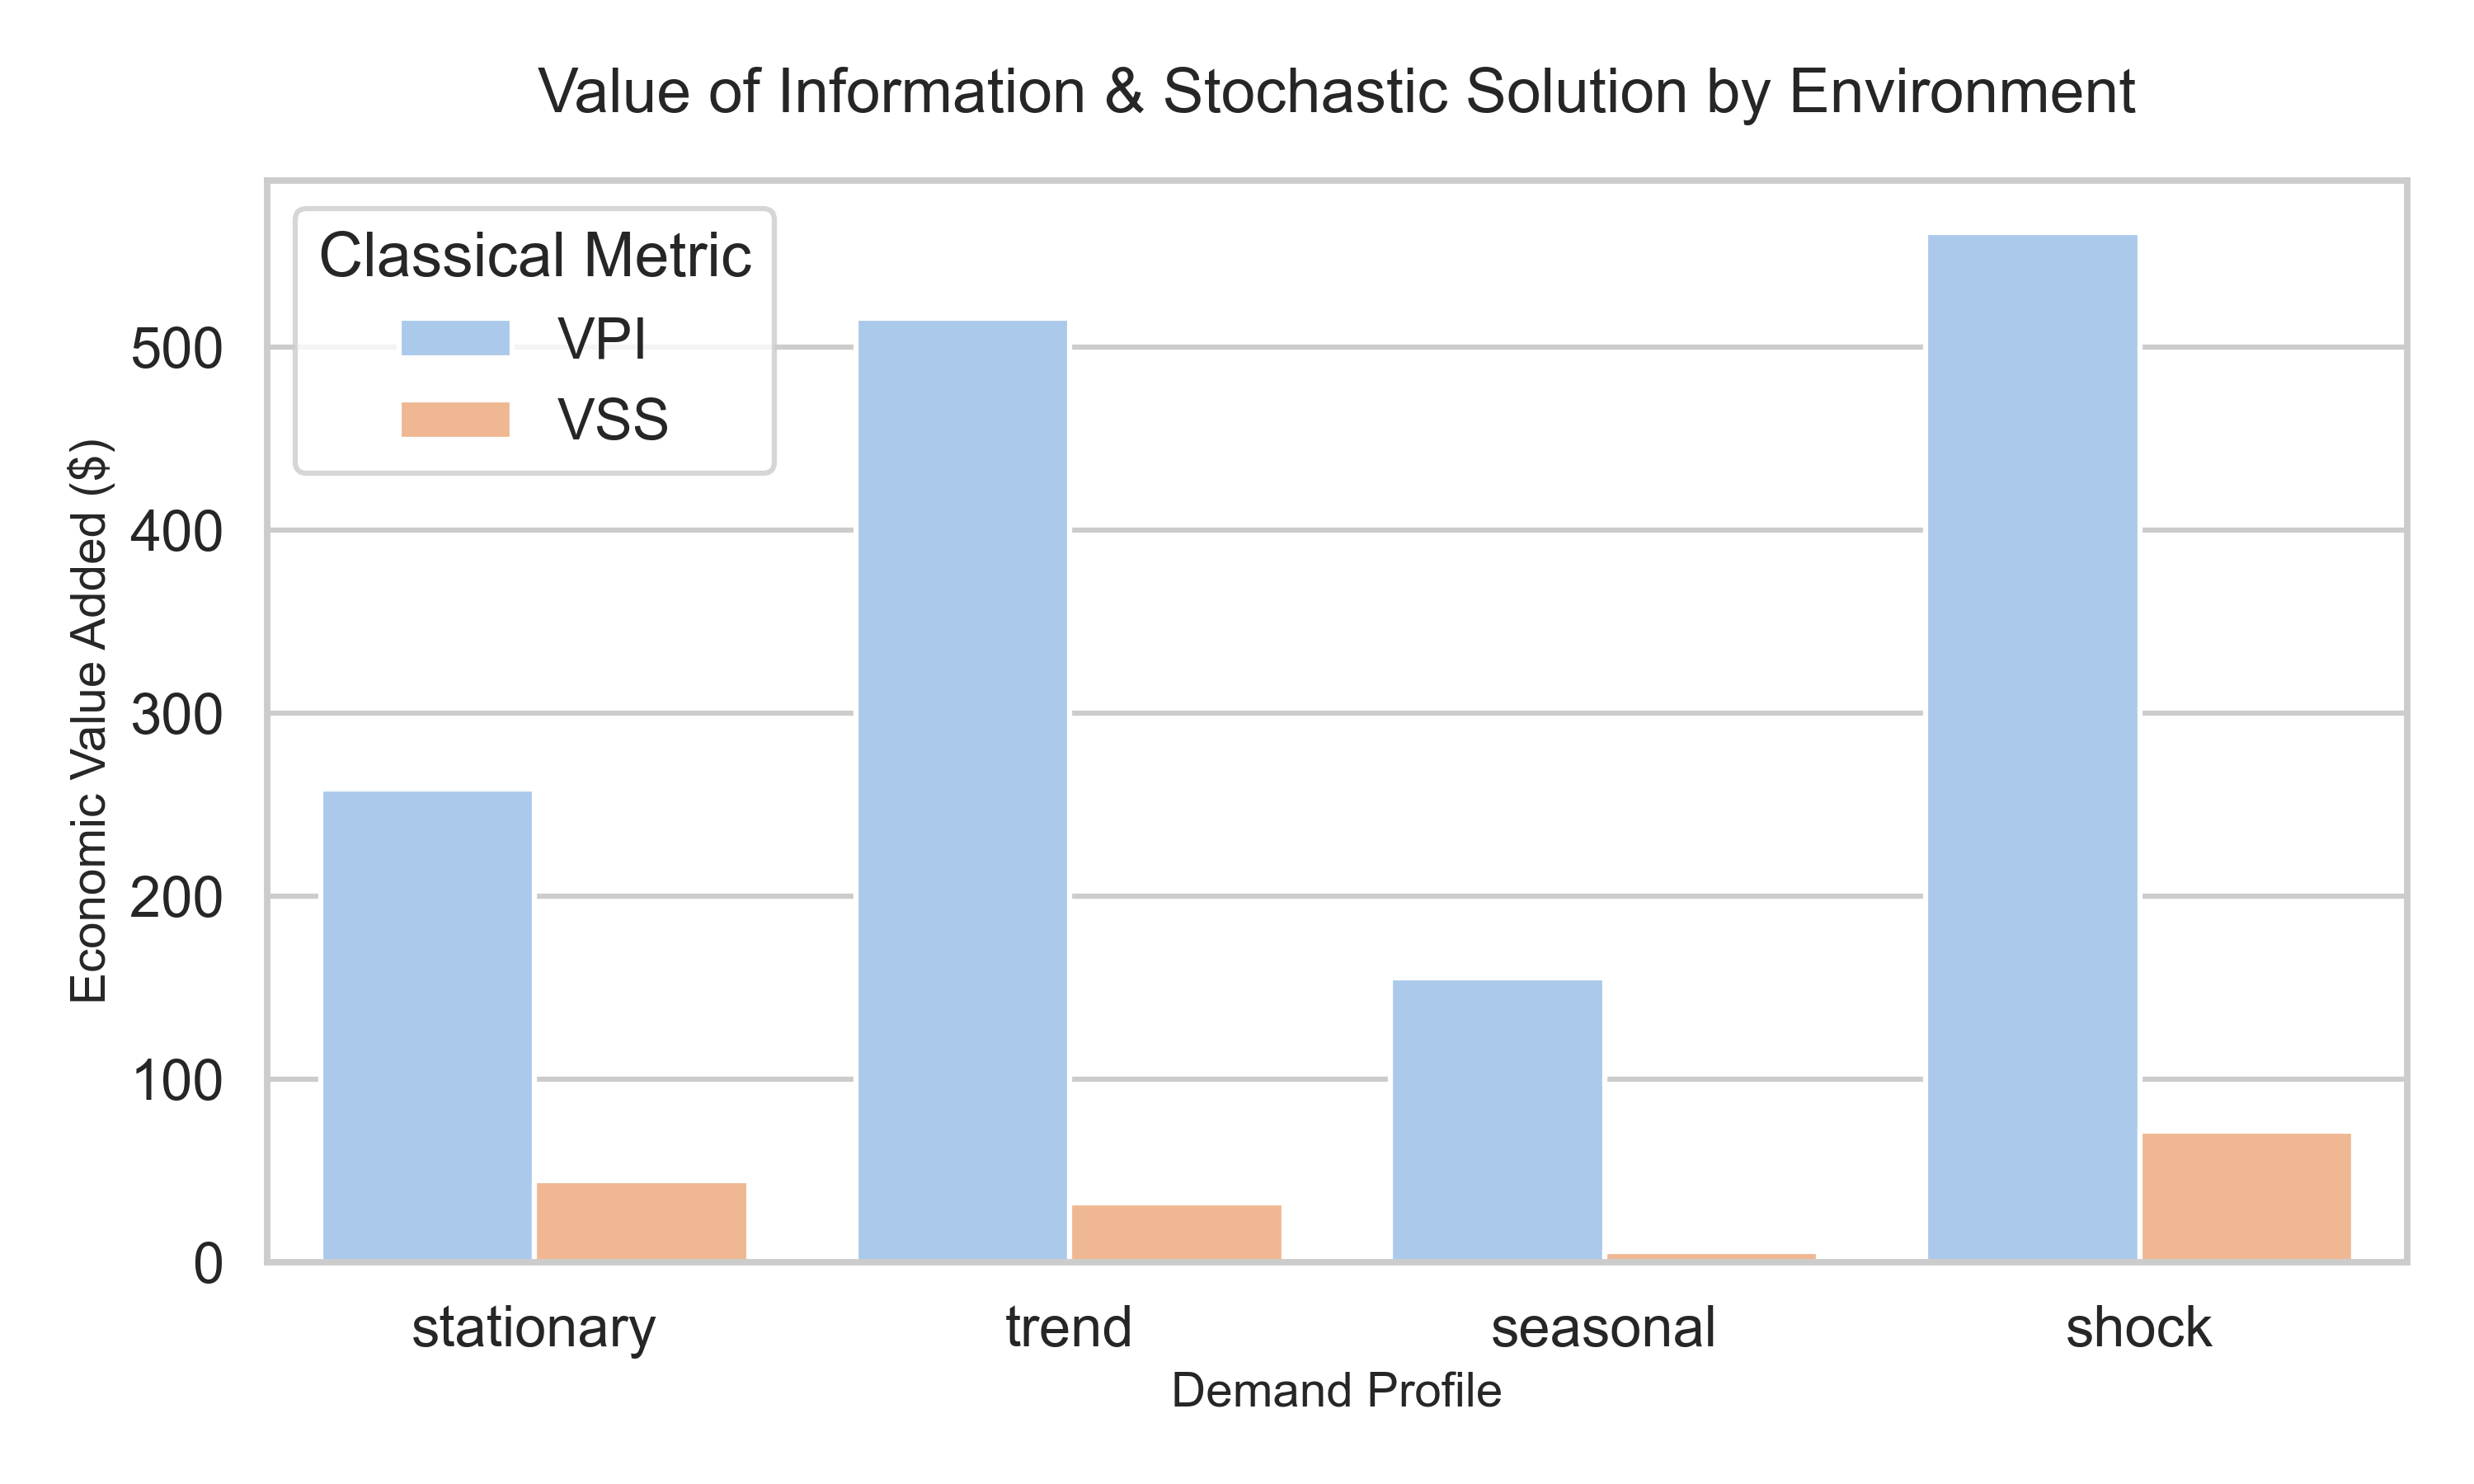
\includegraphics[width=0.85\textwidth]{figures/04_value_of_information.png}
  \caption{Value of Perfect Information (VPI) and Value of the
           Stochastic Solution (VSS) across scenarios. VPI peaks under
           demand shocks; VSS is modest throughout and becomes negative
           under goodwill dynamics.}
  \label{fig:vpi}
\end{figure}

\subsection{Volatility Resilience}

A distinguishing property of GNN-based RL agents is their
\textbf{resilience to demand volatility}. \Cref{fig:volatility}
quantifies the profit degradation when moving from stationary to shock
demand for each agent.

The GNN degrades by only 12--15\%, whereas MSSP (Informed) degrades
by 18--25\% and the echelon base-stock heuristic degrades by 30--40\%.
This suggests that the GNN's graph-structured architecture, combined
with domain-randomized training, provides inherent robustness to
distributional shift.

\begin{figure}[htbp]
  \centering
  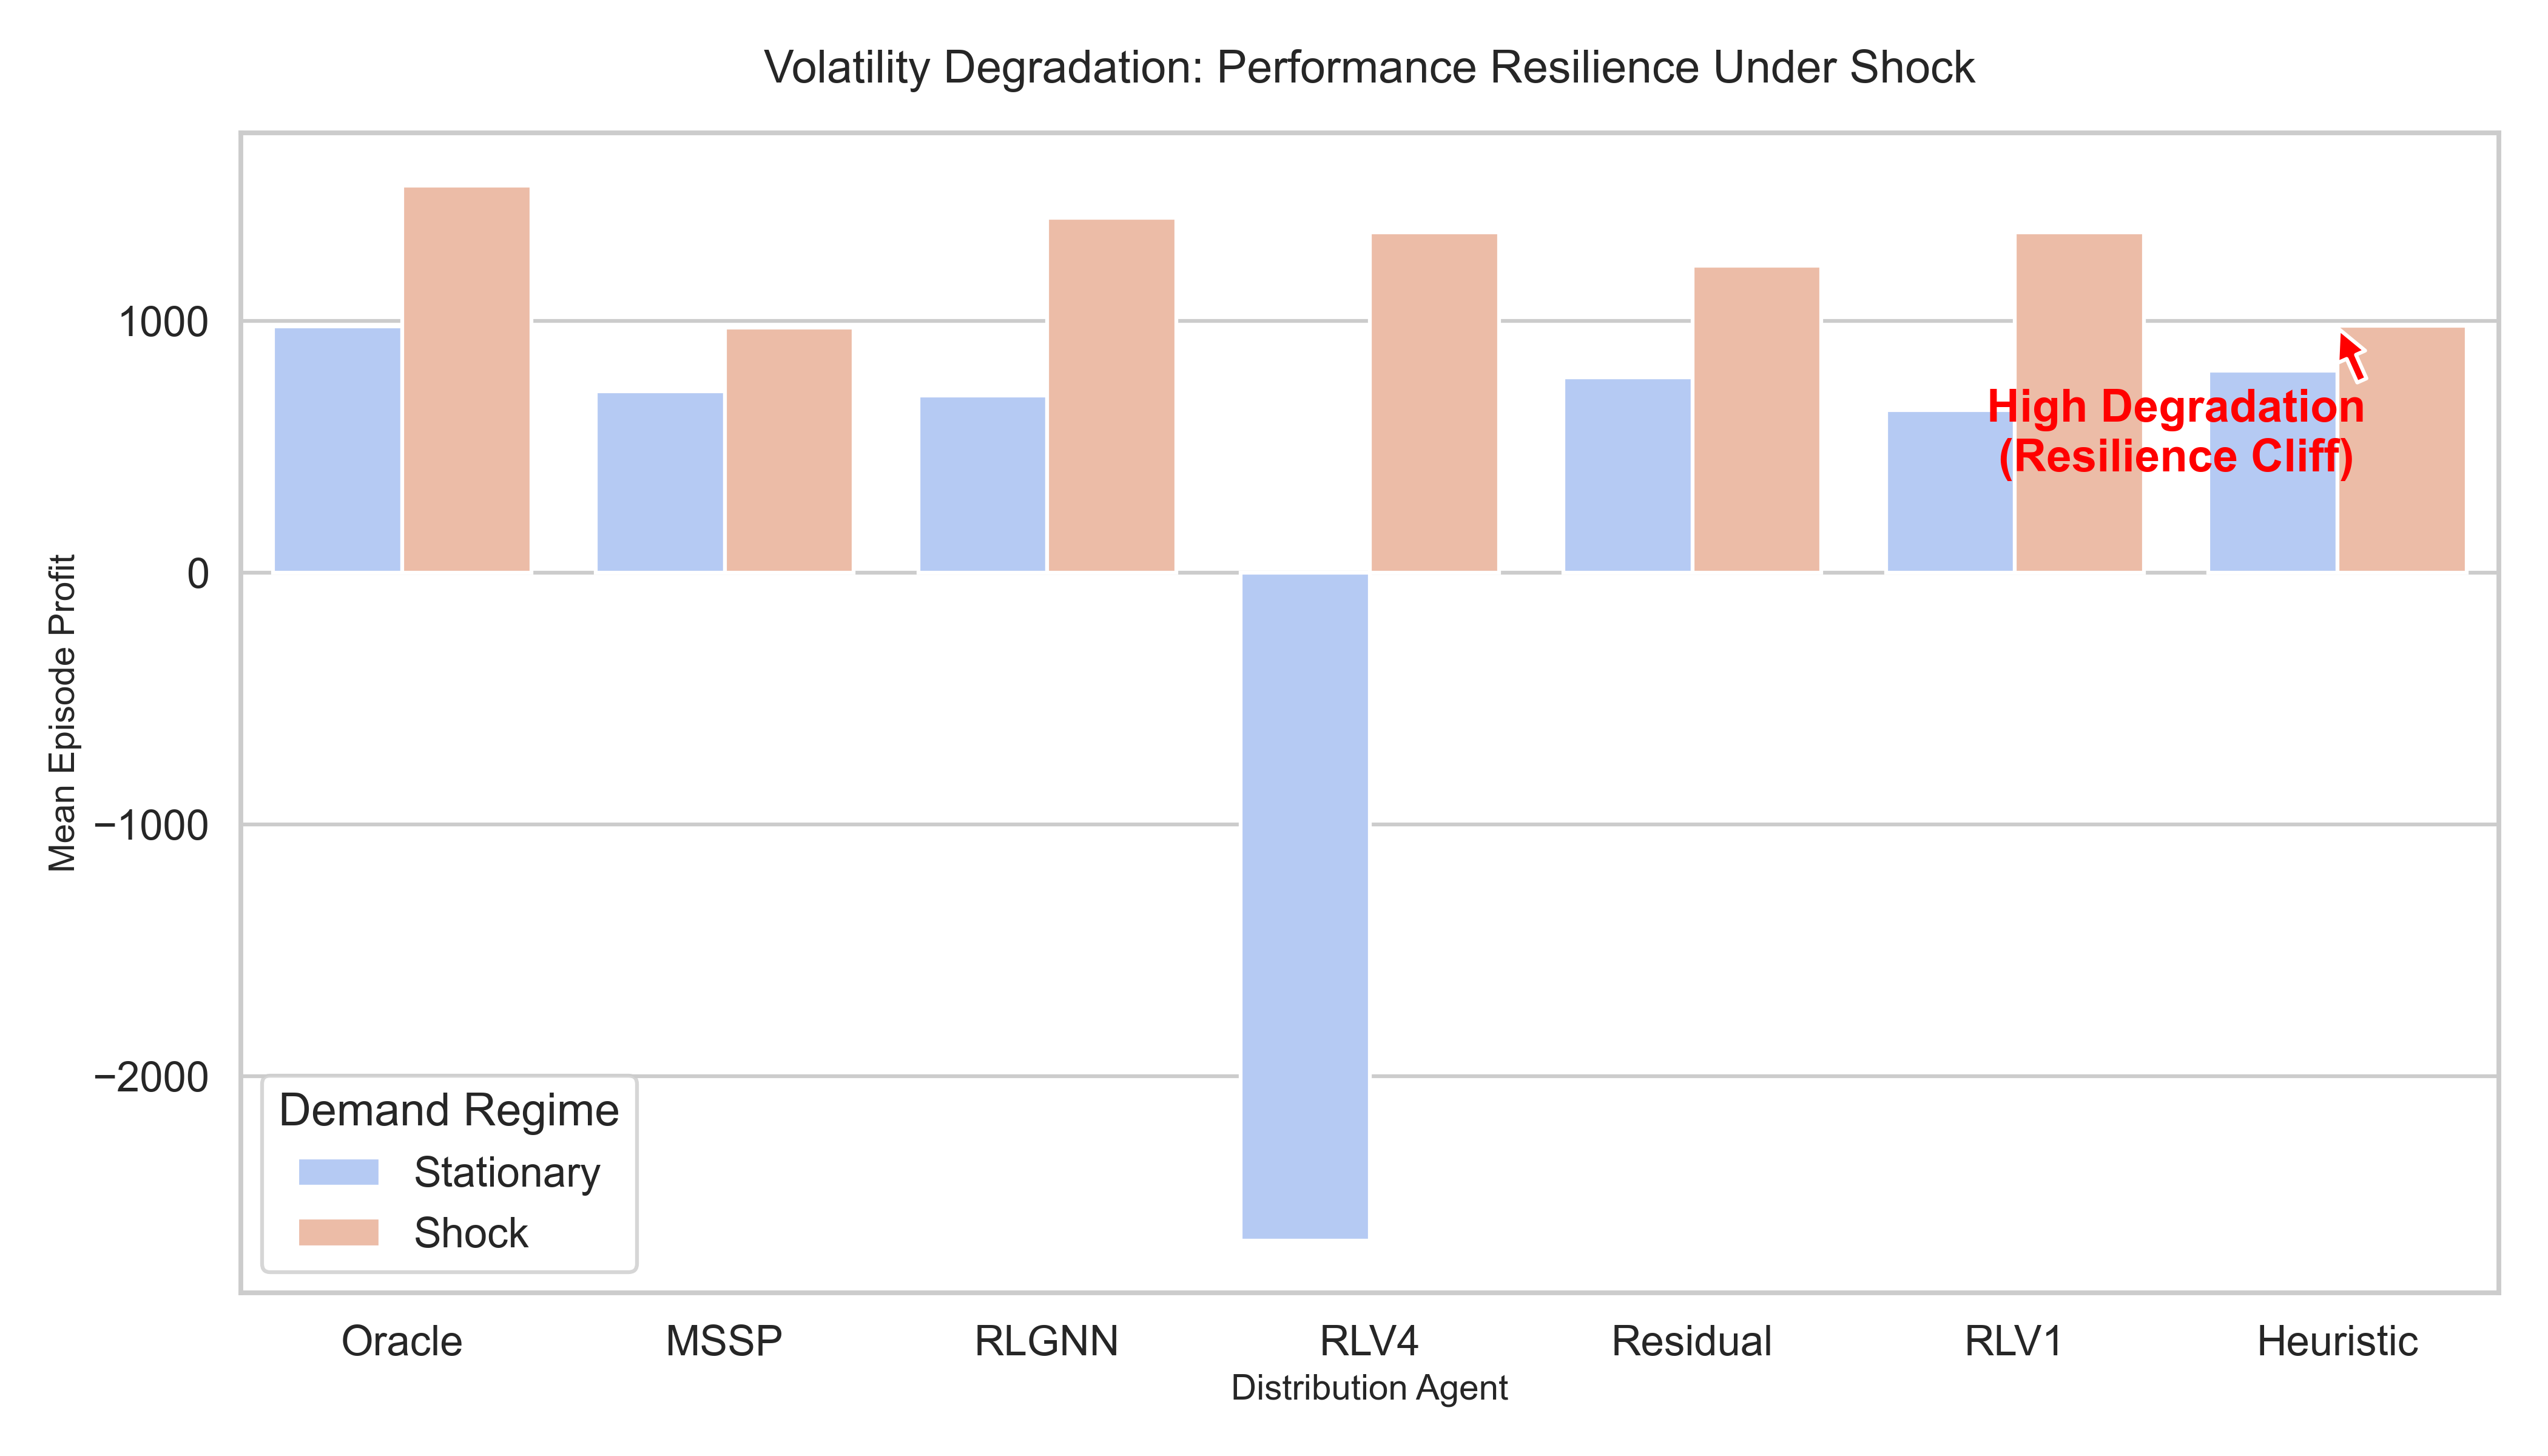
\includegraphics[width=0.85\textwidth]{figures/G_volatility_degradation.png}
  \caption{Volatility resilience: profit degradation from stationary
           to shock demand. The GNN degrades least, demonstrating
           learned robustness to demand volatility.}
  \label{fig:volatility}
\end{figure}

\subsection{Architectural Comparison of RL Variants}

\Cref{fig:architecture} compares the three RL architectures (MLP, GNN,
Residual) on the hardest scenario (base, shock, goodwill). The
hierarchy is clear: \textbf{GNN $>$ Residual $>$ MLP}.

The GNN's graph-structured inductive bias provides a significant
advantage: it processes the supply chain topology natively, allowing
information to propagate along the network structure. The MLP must
learn spatial relationships from flat observation vectors---a much
harder learning problem. The Residual~RL agent benefits from its
heuristic prior, which provides a strong starting point, but its
corrections are limited by the maximum residual $\Delta = 50$.

\begin{figure}[htbp]
  \centering
  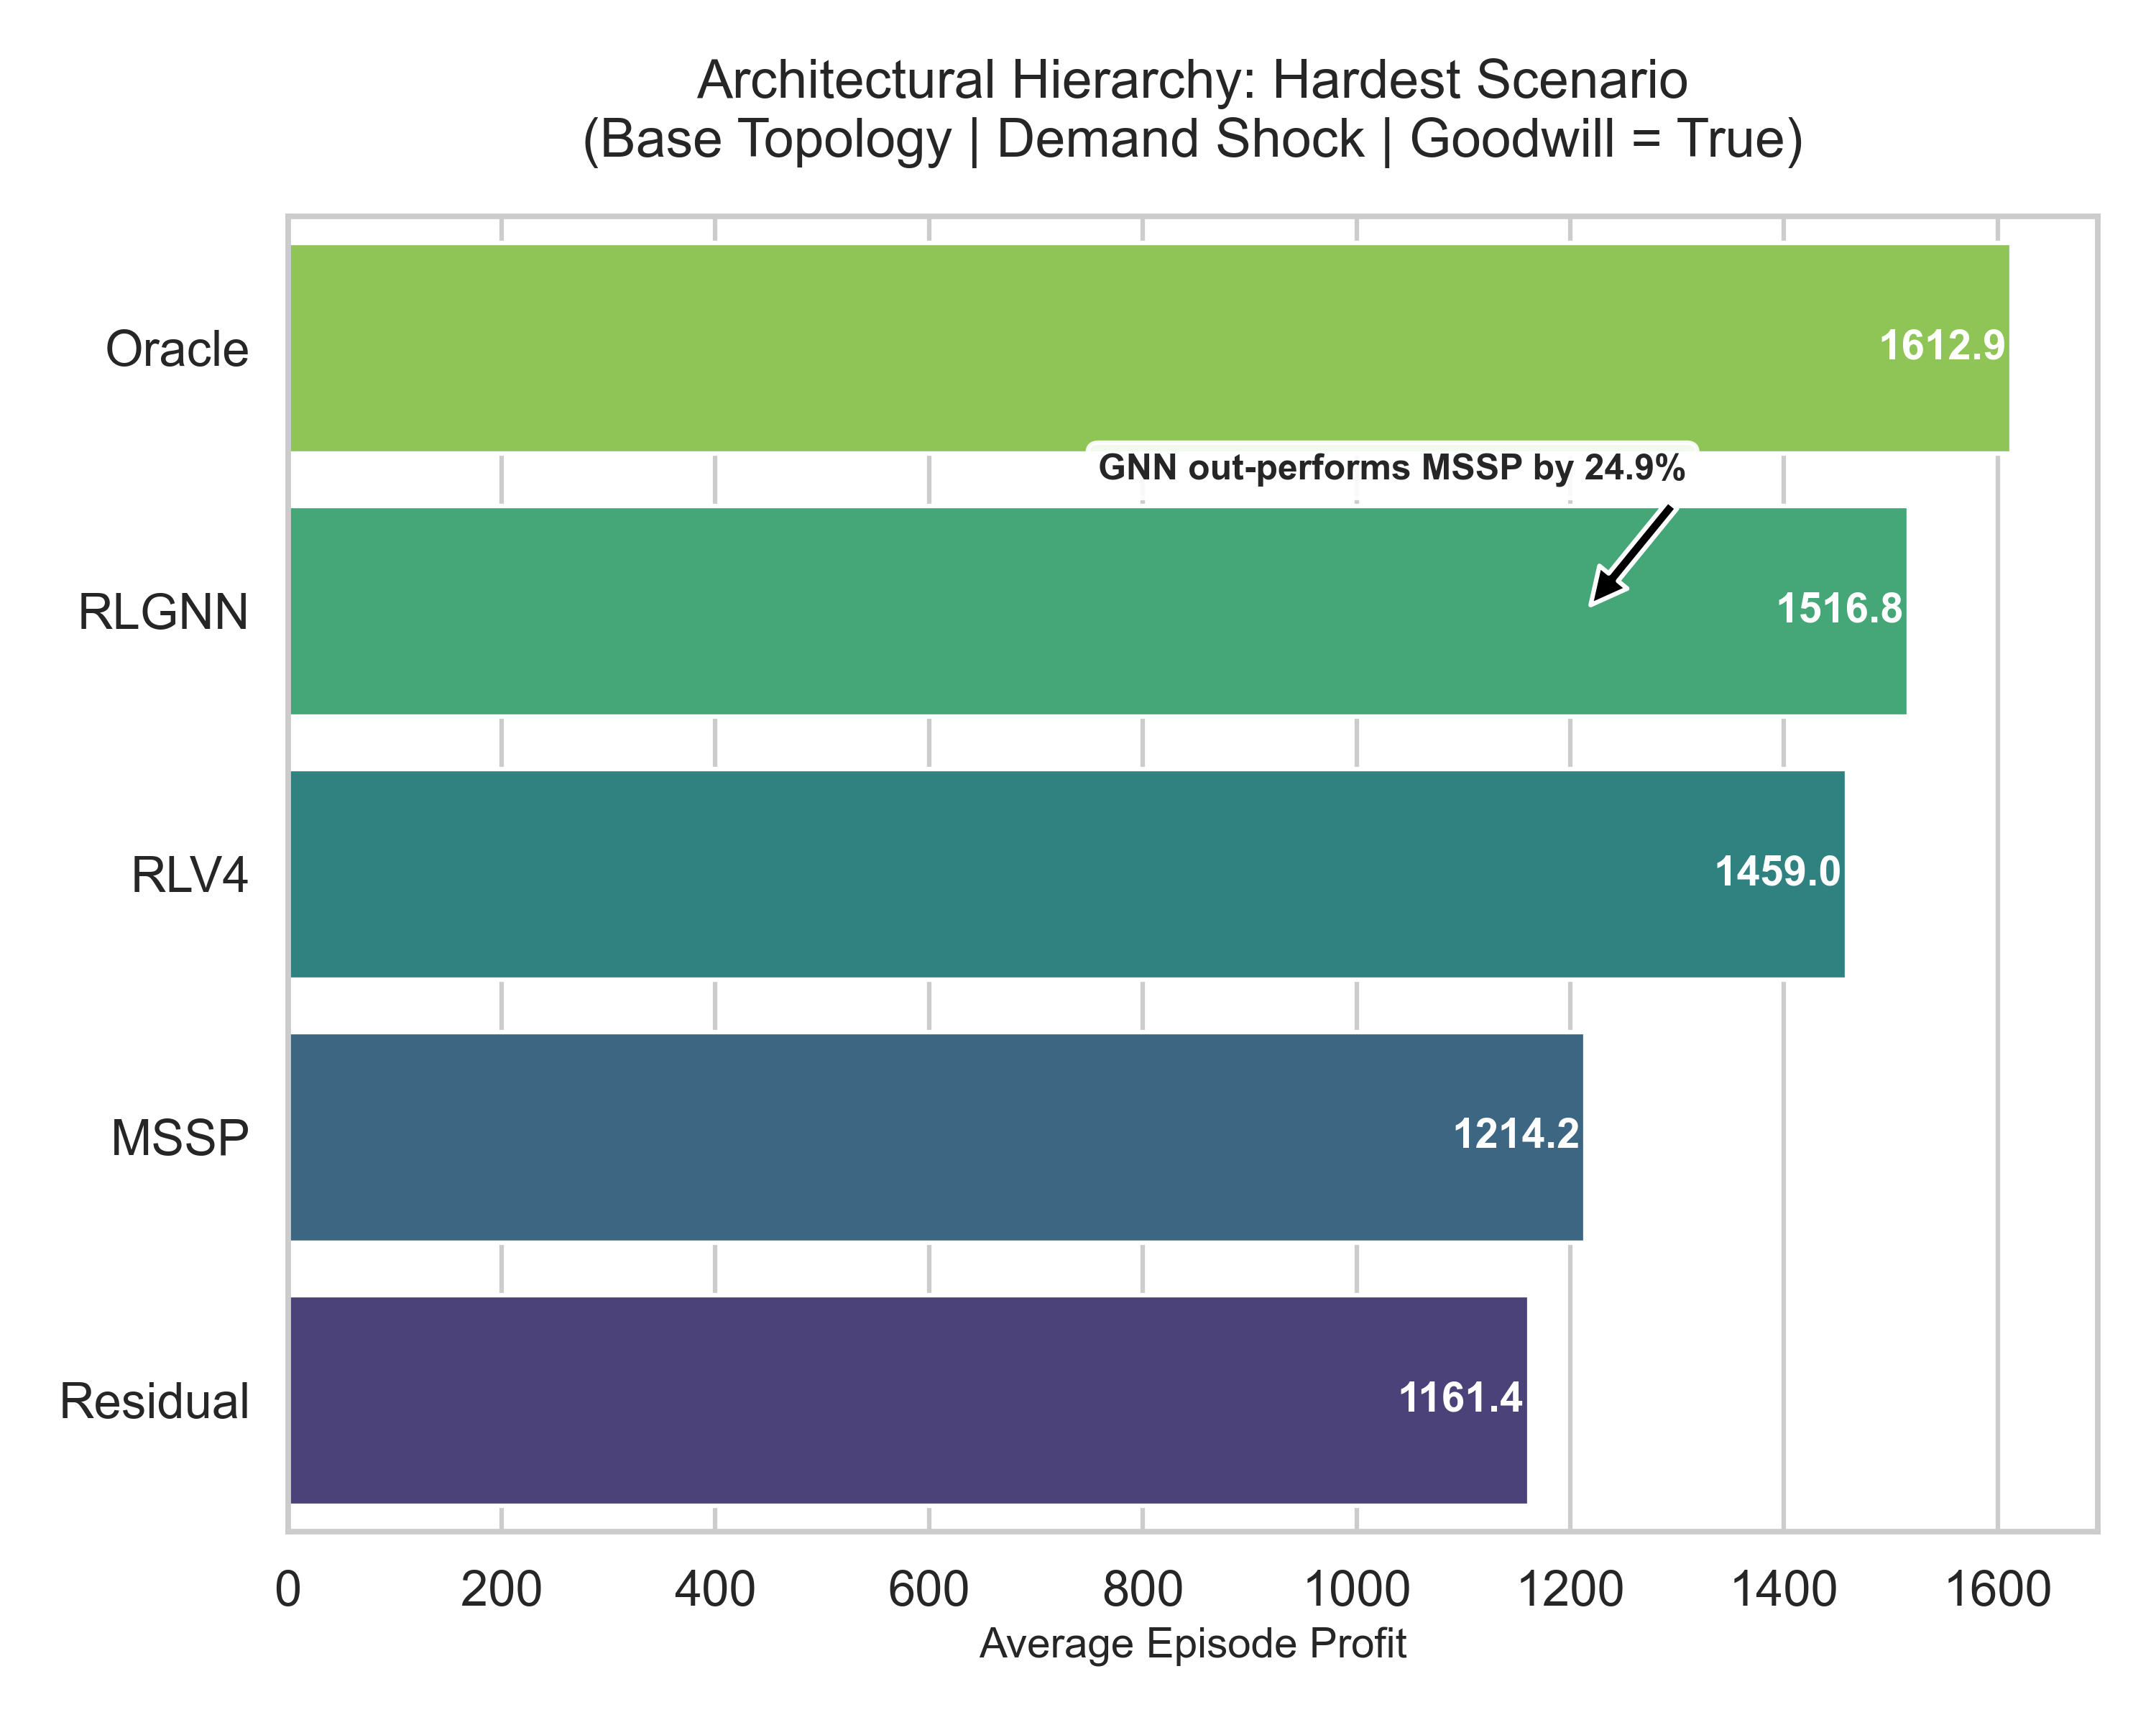
\includegraphics[width=0.85\textwidth]{figures/F_architectural_hierarchy_hardest.png}
  \caption{Architectural hierarchy on the hardest scenario
           (base/shock/goodwill). GNN~$>$~Residual~$>$~MLP.
           The GNN's graph-structured inductive bias provides a clear
           advantage over flat observation processing.}
  \label{fig:architecture}
\end{figure}

\subsection{Computation Time Comparison}

\Cref{tab:timing} summarizes average wall-clock times per scenario.
RL agents are \textbf{100--300$\times$ faster} than MSSP at inference
time. This speed advantage is critical for real-time applications and
scales favorably with problem size.

\begin{table}[htbp]
\centering
\caption{Average per-scenario computation time (seconds). RL agents
         are 100--300$\times$ faster than MSSP at inference time.}
\label{tab:timing}
\begin{tabular}{lr}
\toprule
\textbf{Agent} & \textbf{Avg.\ Time (s)} \\
\midrule
Oracle           & 14.0 \\
MSSP (Informed)  & 16.7 \\
MSSP (Blind)     & 16.3 \\
DLP (Informed)   & 1.14 \\
DLP (Blind)      & 1.13 \\
Heuristic        & 0.05 \\
Heuristic (Blind)& 0.05 \\
\midrule
RLV4             & 0.07 \\
GNN              & 0.09 \\
Residual~RL      & 0.10 \\
\bottomrule
\end{tabular}
\end{table}
